% 2006 天津文科 Q22，源：固定 PDF 第 2 页（印刷页 339）。
% 几何比例依题面推出的 x^2-4y^2=1 作示意；以 m=3/4、参数 p=1/10 为一组
% 可行示例定位 A,B,C,D,E。拓扑：渐近线过 O；左准线过 M；DE 竖直；l 为 D-A-C，
% BC 为 E-C-B。其余焦点位置按 F1,F2=(±sqrt(5)/2,0)。
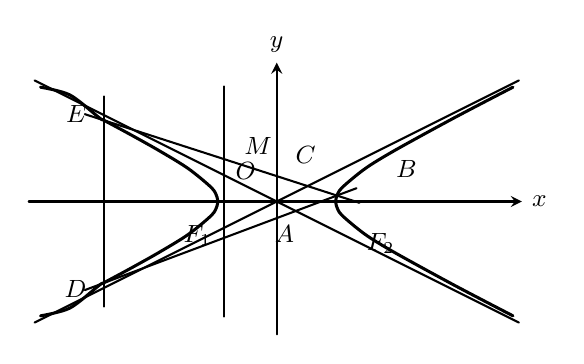
\begin{tikzpicture}[x=0.75cm,y=0.75cm,line cap=round,line join=round,line width=0.75pt,font=\small,>=stealth]
  % 坐标轴
  \draw[->] (-4.2,0)--(4.15,0) node[right] {$x$};
  \draw[->] (0,-2.25)--(0,2.35) node[above] {$y$};

  % 左准线 x=-2/sqrt(5)，及同一竖直线上的 D、E
  \draw (-0.894,-1.95)--(-0.894,1.95);
  \draw (-2.922,-1.78)--(-2.922,1.78);

  % 双曲线 x^2-4y^2=1
  \draw[line width=1.1pt] plot[smooth] coordinates {
    (-4,1.936) (-3.5,1.803) (-3,1.414) (-2.922,1.373)
    (-2.5,1.146) (-2,0.866) (-1.5,0.559) (-1.1,0.229)
    (-1.01,0.071) (-1,0)
  };
  \draw[line width=1.1pt] plot[smooth] coordinates {
    (-4,-1.936) (-3.5,-1.803) (-3,-1.414) (-2.922,-1.373)
    (-2.5,-1.146) (-2,-0.866) (-1.5,-0.559) (-1.1,-0.229)
    (-1.01,-0.071) (-1,0)
  };
  \draw[line width=1.1pt] plot[smooth] coordinates {
    (1,0) (1.01,0.071) (1.1,0.229) (1.5,0.559)
    (2,0.866) (3,1.414) (4,1.936)
  };
  \draw[line width=1.1pt] plot[smooth] coordinates {
    (1,0) (1.01,-0.071) (1.1,-0.229) (1.5,-0.559)
    (2,-0.866) (3,-1.414) (4,-1.936)
  };

  % 渐近线，以及 l=D-A-C、BC=E-C-B
  \draw (-4.1,2.05)--(4.1,-2.05);
  \draw (-4.1,-2.05)--(4.1,2.05);
  \draw (-3.25,-1.5)--(1.35,0.225);
  \draw (-3.25,1.479)--(1.4,-0.022);

  % 关键点（示意参数 m=3/4,p=1/10）
  \node[left] at (-3.05,1.48) {$E$};
  \node[left] at (-3.05,-1.48) {$D$};
  \node[above right] at (-0.72,0.62) {$M$};
  \node[below] at (-1.34,-0.24) {$F_1$};
  \node[above left] at (-0.18,0.20) {$O$};
  \node[below left,xshift=-6pt,yshift=-5pt] at (0.75,0) {$A$};
  \node[above left,xshift=-4pt,yshift=8pt] at (1.02,0.101) {$C$};
  \node[below right,xshift=5pt,yshift=-8pt] at (1.118,0) {$F_2$};
  \node[above right,xshift=11pt,yshift=5pt] at (1.333,0) {$B$};
\end{tikzpicture}
